\documentclass[16pt,a4paper]{jsarticle}
\title{連続系アルゴリズム レポート課題13}
\author{161015 佐藤 友哉}
\date{}
\usepackage{listings, jlisting}
\usepackage{amsmath}
\lstset{%
  language={C},
  basicstyle={\small},%
  identifierstyle={\small},%
  commentstyle={\small\itshape},%
  keywordstyle={\small\bfseries},%
  ndkeywordstyle={\small},%
  stringstyle={\small\ttfamily},
  frame={tb},
  breaklines=true,
  columns=[l]{fullflexible},%
  numbers=left,%
  xrightmargin=0zw,%
  xleftmargin=3zw,%
  numberstyle={\scriptsize},%
  stepnumber=1,
  numbersep=1zw,%
  lineskip=-0.5ex%
}
\usepackage[dvipdfmx]{graphicx}
\begin{document}
\maketitle
\section*{課題5}
\subsection*{問題1}
Legendre多項式の$P_0$から$P_3$までの導出
\subsubsection*{$P_0$の導出}
\begin{eqnarray}
  \int_{-1}^{1} {P_0}^2 dx\ &=&\ 2 \nonumber \\
  P_0\ =\ 1 \nonumber
\end{eqnarray}
\subsubsection*{$P_1$の導出}
$P_1(x) = Ax + B$とおく
\begin{eqnarray}
  \int_{-1}^{1} (Ax + B) dx\ &=&\ 0 \nonumber \\
  \int_{-1}^{1} (Ax + B)^2 dx\ &=&\ \frac{2}{3} \nonumber
\end{eqnarray}
これを満たす$A,B$は$A = 1$, $B = 0$
よって$P_1(x) = x$
\subsubsection*{$P_2$の導出}
$P_2(x) = Ax^2 + Bx + C$とおく
\begin{eqnarray}
  \int_{-1}^{1} (Ax^2 + Bx + C) dx\ &=&\ 0 \nonumber \\
  \int_{-1}^{1} (Ax^2 + Bx + C)x dx\ &=&\ 0 \nonumber \\
  \int_{-1}^{1} (Ax^2 + Bx + C)^2 dx\ &=&\ \frac{2}{5} \nonumber
\end{eqnarray}
これを満たす$A,B,C$は$A = \frac{3}{2}, B = 0, C = - \frac{1}{2}$
よって$P_2(x) = \frac{3}{2} x^2 - \frac{1}{2}$
\subsubsection*{$P_3$の導出}
$P_3(x) = Ax^3 + Bx^2 + Cx + D$とおく
\begin{eqnarray}
  \int_{-1}^{1} (Ax^3 + Bx^2 + Cx + D) dx\ &=&\ 0 \nonumber \\
  \int_{-1}^{1} (Ax^3 + Bx^2 + Cx + D)x dx\ &=&\ 0 \nonumber \\
  \int_{-1}^{1} (Ax^3 + Bx^2 + Cx + D)(\frac{3}{2}x^2 - \frac{1}{2}) dx\ &=&\ 0 \nonumber \\
  \int_{-1}^{1} (Ax^3 + Bx^2 + Cx + D)^2 dx\ &=&\ \frac{2}{7} \nonumber
\end{eqnarray}
第1・3式より$B = D = 0$が分かり、残りの式から$A = \frac{5}{2}, C = -\frac{3}{2}$がわかる。よって$P_3(x) = \frac{5}{2}x^3 - \frac{3}{2}x$
\subsection*{問題2}
chebyshev多項式の漸化式による数値計算
$P_1 = x, P_2 = 2x^2 - 1$を元に漸化式$P_{k+2} = 2x P_{k+1} - P_k$によって$P_5$まで求めgnuplotによってグラフを描画するc言語プログラムを作成した。
\begin{figure}[h]
  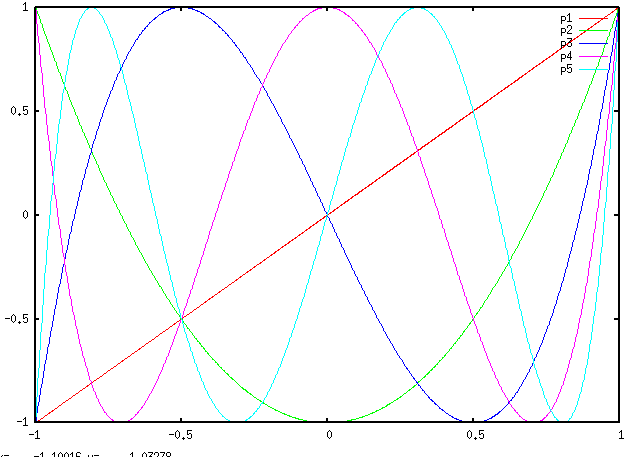
\includegraphics[width=15.0cm]{chev.png}
\end{figure}
\lstinputlisting[caption=CHEBYSHEV, label=CHEBYSHEV]{che.c}
\section*{課題8}
\subsection*{問題1}
${l_i},{d_i},{u_i}$を求める式
\begin{eqnarray}
  b_k\ &=&\ u_k \nonumber \\
  a_k\ &=&\ d_k\ +\ u_{k-1}l_k \nonumber \\
  c_k\ &=&\ d_{k-1}l_k \nonumber
\end{eqnarray}
n×n行列に対してn回この式を繰り返し、この式を解く計算量は定数回なので全体としての計算量はO(n)となる
\subsection*{問題2}
c言語による実装。最初に行列サイズn,m,lをint型としてscanfで受け取りn×m行列とm×l行列を二次元配列で受け取るためにメモリ領域を動的に確保する。その後各行列の要素をfloat型としてscanfで受け取ると自動で積を計算する。

\lstinputlisting[caption=MULTIPLE,label=MULTIPLE]{rp8.c}
\end{document}
